\documentclass{beamer}
%
% Choose how your presentation looks.
%
% For more themes, color themes and font themes, see:
% http://deic.uab.es/~iblanes/beamer_gallery/index_by_theme.html
%
\mode<presentation>
{
  \usetheme{Warsaw}      % or try Darmstadt, Madrid, Warsaw, ...
  \usecolortheme{default} % or try albatross, beaver, crane, ...
  \usefonttheme{structurebold}  % or try serif, structurebold, ...
  \setbeamertemplate{navigation symbols}{<= =>}
  \setbeamertemplate{caption}[numbered]
} 

\usepackage[english]{babel}
\usepackage[utf8x]{inputenc}
\usepackage{ragged2e}
\justifying

\title[Imagelib \hspace{25mm} \insertframenumber /20 ]{Imagelib}

\author{Erick Eduarte. \and  Luis Felipe Rincón. \and Fabián Meléndez.}
\institute{Universidad de Costa Rica}
\date{07/10/2013}

\section{Introducción}
\subsection{Introducción}

\begin{document}

\begin{frame}
  \titlepage
\end{frame}




\begin{frame}{Introducción}

Este trabajo se basa en crer una librería que aplica distintos filtros y funciones básicas a una imagen, ya sea monocromática (En escala de grises) o RGB, que se refiere a una imagen de 3 capas roja, verde y azul.


  \begin{block}{Definición}
  \justifying
 Una imagen digital es el conjunto de elementos de una función bidimensional (x,y), que además cada par son coordenadas espaciales que tienen asociada una intensidad, y son llamados píxeles.
 \end{block}


\end{frame}

\subsection{Procesamiento de Imágenes}



\begin{frame}{Procesamiento de Imágenes}

  \begin{block}{Definición}
  \justifying
  El procesamiento digital de imágenes es el conjunto de técnicas que se aplican a las imágenes digitales con el objetivo de mejorar la calidad o facilitar la búsqueda de información.
  \end{block}
  

\large{Usos:}
\begin{itemize}

\item Eliminar/Disminuir Ruido.
\item Resaltar detalles.
\item Detectar Bordes.
\item Extraer Información

\end{itemize}

\end{frame}


\begin{frame}{Aplicaciones}

\begin{itemize}

\item Medicina (Gamografía ósea y rayos X)
\item Astronomía (Ciclo de Cygnus)
\item Industria (Electrónica)
\item Biología (Microscopía)
\item Climatología (Fenómenos atmosféricos)
\item Identificación o conteo de objetos

\end{itemize}

\end{frame}



\begin{frame}{Imágen Digital}

Una imagen es una representacion visual y bidimensional de un objeto. Matemáticamente puede ser descrita como:

\begin{center}
\begin{math}
	\centering
	$f(x,y)=$
   \begin{pmatrix} 
    f(0,0) & f(0,1) & ... & f(0,N) \\ 
 	f(1,0) & f(1,1) & ... & f(1,N) \\
    \vdots & \vdots & \ddots & \vdots \\

    f(M,0) & (M,1) & ... & f(M,N) \\
   \end{pmatrix}
\end{math}\\
\end{center}


\end{frame}

\begin{frame}{Filtro}

Es una transformacion, de una imagen original, para resaltar o mejorar detalles de la imagen, suavizarla o resaltar bordes, asi como para disminuir el ruido. 
\begin{columns}
\column[t]{5cm}
\begin{center}
\begin{math}
g(x,y) = T[f(x,y)] 
\end{math}\\

\begin{math}
\begin{pmatrix}
	z_1 & z_2 & z_3 \\
    z_4 & z_5 & z_6 \\
    z_7 & z_8 & z_9 \\
\end{pmatrix}
\end{math}
\end{center}

\column[t]{5cm}

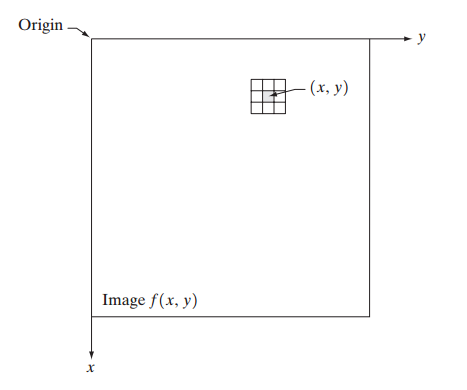
\includegraphics[scale=0.25]{./.Presentation/filter.png}

\end{columns}

\begin{block}{Definición}
\begin{center}
\begin{math}
	g(x,y) = f(x-1,y-1)\cdot z_1 + f(x, y-1) \cdot z_2 + f(x+1,y-1)\cdot z_3 + f(x-1, y) \cdot z_4 + f(x,y) \cdot z_5 + f(x+1,y) \cdot z_6 + f(x-1, y+1) \cdot z_7 + f(x, y+1) \cdot z_8 + f(x+1, y+1) \cdot z_9
\end{math}
\end{center}
\end{block}
\end{frame}




\section{Imagelib}



\begin{frame}{Imagelib}

\begin{block}{Imagelib}
Librería para el procesamiento de Imágenes.
\end{block}

\begin{itemize}
\item Operaciones Aritmeticas y Lógicas.
\item Filtros en el dominio espacial.
  \item Filtros Suavizantes.
  \item Filtros Constrastantes.
\item Procesamiento de Histogramas.
\item Transformaciones Punto a Punto.
\item Funciones Estadísticas.

\end{itemize}


\end{frame}






% 2 Aritmeticas y Logicas
% 2 Suavizantes
% 2 constrastantes
% 2 trasnformaciones punto a punto
% 2 estadisticas
% 1 Histogramas
% 1 Ruido
% 1 Orientadas




\subsection{Filtros en el dominio del espacio}


\begin{frame}{Operaciones Aritméticas}
\begin{columns}

\column[t]{5.9cm}
\begin{center}
\begin{block}{Suma}
Suma los píxeles de dos imágenes de las mismas dimensiones. Es útil para superponer dos imágenes.
\end{block}
\vspace{0.5cm}
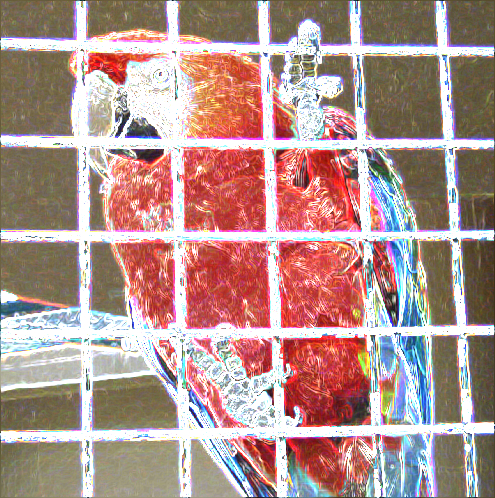
\includegraphics[scale=0.15]{./.Presentation/parrot_sum}
\end{center}

\column[t]{5.9cm}
\begin{center}
\begin{block}{Resta}
Resta los píxeles de dos imágenes de las mismas dimensiones. Es utilizado para ver las diferencias entre 2 imágenes. 
\end{block}
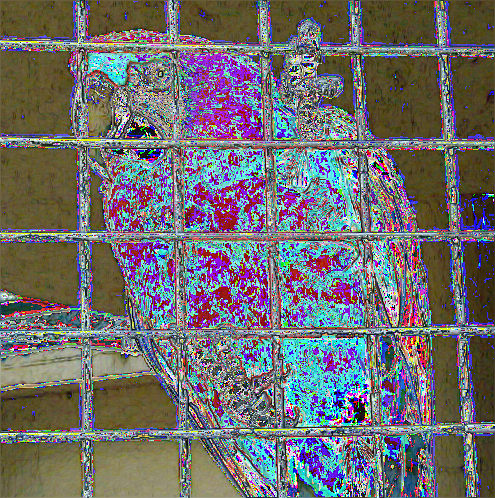
\includegraphics[scale=0.15]{./.Presentation/parrot_substracted}
\end{center}
\end{columns}

\end{frame}

\begin{frame}{Operaciones Aritméticas}
\begin{columns}
\column[t]{5.9cm}
\begin{center}
\begin{block}{Multiplicación}
\justifying

Consiste en multiplicar los píxeles de una imagen por un factor para aumentar o disminuir su intensidad.
\end{block}
\vspace{0.5cm}
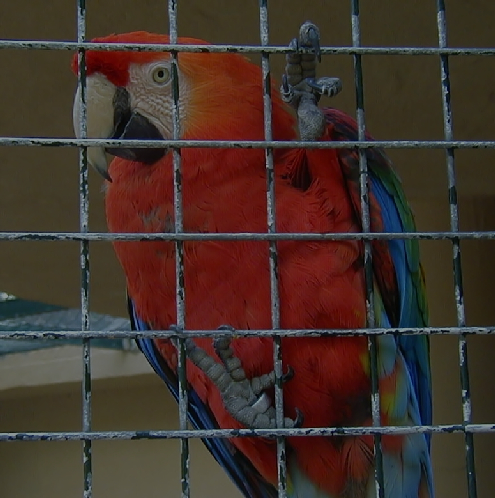
\includegraphics[scale=0.15]{./.Presentation/parrot_multiplied}
\end{center}

\column[t]{5.9cm}
\begin{center}
\begin{block}{Binarización}
\justifying

Toma los píxeles mayores a un valor de corte y se ajustan al máximo de intensidad y los que se encuentran por debajo, al mínimo.
\end{block}
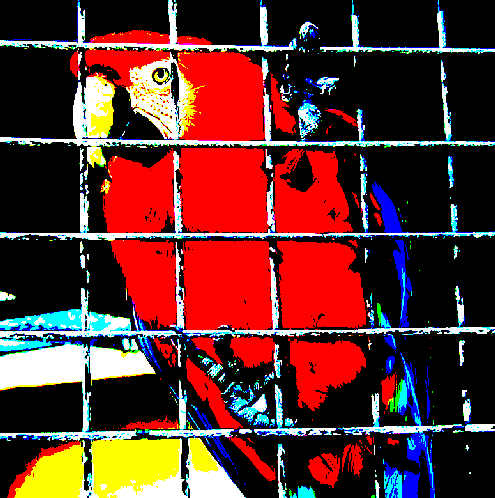
\includegraphics[scale=0.15]{./.Presentation/parrot_binarized}
\end{center}
\end{columns}
\end{frame}

\begin{frame}{Suavización}

Los filtros de suavización o paso pajo atenuan las altas frecuencias. Se utilizan para minimizar los ruidos y detalles de la imagen, haciéndola menos nítida.
\begin{columns}
\column[t]{5cm}
\begin{block}{Promedio}
\justifying
Calcula la media de los valores de los pixeles en la máscara para reducir cambios abruptos de intensidad.
\end{block}
\column[t]{5cm}

\begin{block}{Mediana}
\justifying
Calcula la mediana entre los pixeles circundantes y la aplica al pixel central del kernel.
\end{block}
\end{columns}

\end{frame}


\begin{frame}{Suavización}

\begin{columns}
\column[t]{5cm}
\begin{block}{Moda}
\justifying
Encuentra el valor de mayor frecuencia entre la vencidad de pixeles de una región y lo aplica.
\end{block}

\begin{block}{Filtro Gaussiano}
\justifying
Aplica una convolución de la imagen con un kernel gaussiano.
\begin{math}
G_{\sigma}(x,y)=\frac{1}{\sqrt{2\pi\sigma^2}}e^\frac{-(x^2+y^2)}{2\sigma^2}
\end{math}
\end{block}

\column[t]{5cm}

\begin{center}
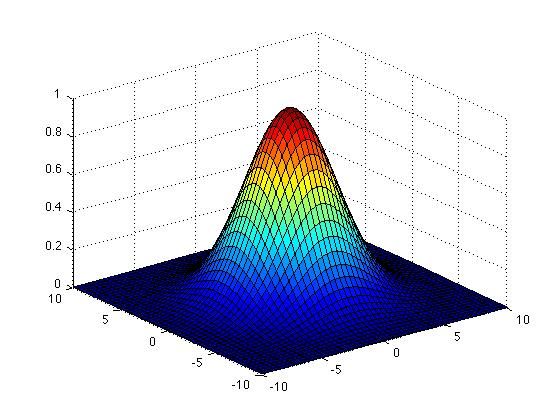
\includegraphics[scale=0.30]{./.Presentation/gauss.jpg}
\end{center}

\end{columns}
\end{frame}

\begin{frame}{Contrastación}

 Se utilizan para detectar cambios de intensidad, y des-enfatizar zonas donde la intensidad sea casi constante. Se utilizan para la detección de bordes. Algunos ejemplos de filtros contrastantes son: 
 
 \begin{itemize}
 \item Laplaciano
 \item Gradiente
 \item Prewitt
 \item Desplazamiento y diferencia.
 \item Bordes Horizontales y Verticales
 \end{itemize}
\end{frame}

\begin{frame}{Contrastación}
\begin{columns}
\column[t]{5cm}

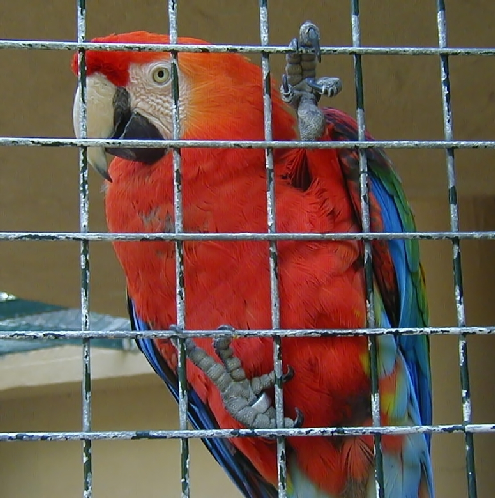
\includegraphics[scale=0.18]{./.Presentation/parrot_original} \\
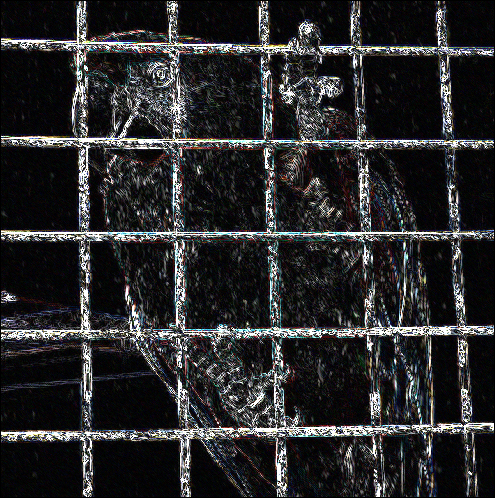
\includegraphics[scale=0.18]{./.Presentation/parrot_laplace} \\

\column[t]{5cm}

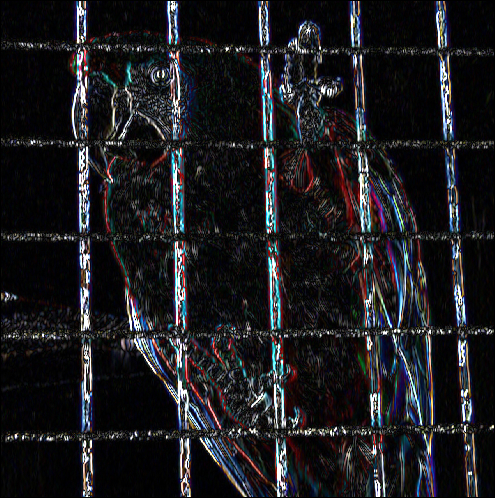
\includegraphics[scale=0.18]{./.Presentation/parrot_EW} \\
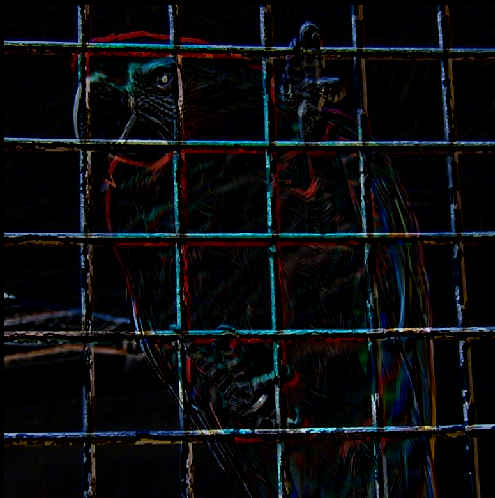
\includegraphics[scale=0.18]{./.Presentation/parrot_displaced2}

\end{columns}
\end{frame}


\subsection{Otros Métodos}

\begin{frame}{Transformaciones punto a punto}
\begin{columns}
\column[t]{6.5cm}
\begin{block}{Dilatación del Rango Dinámico}
\begin{math}
v= \left\{
	\begin{array}{cl}
		u\alpha & \mbox{si } 0<u<a\\
		\beta(u-a)+v_a &\mbox{si } a\leq u<b\\
	\gamma(u-b)+v_b &\mbox{si } b\leq u\leq L\\
	\end{array}\right.
\end{math}
\end{block}

\column[t]{5cm}
\begin{block}{Negativo de una Imagen}
\justifying
Consiste ajustar el valor del píxel a la resta del valor máximo de intensidad con el valor actual del píxel.
\end{block}
\end{columns}

\begin{block}{\begin{center}Transformación a Potencia\end{center}}
\begin{center}
\begin{math}
g(x,y) = k \cdot \left( f(x,y) )^{\gamma} \right)
\end{math}
\end{center}
\end{block}

\end{frame}

\begin{frame}{Transformaciones punto a punto}
\begin{columns}
\column[t]{5cm}
\begin{center}
\begin{block}{Transformación Logarítmica} 

\begin{math}
	v = c \cdot log (u + 1)
\end{math}
\end{block}
\end{center}

\begin{center}
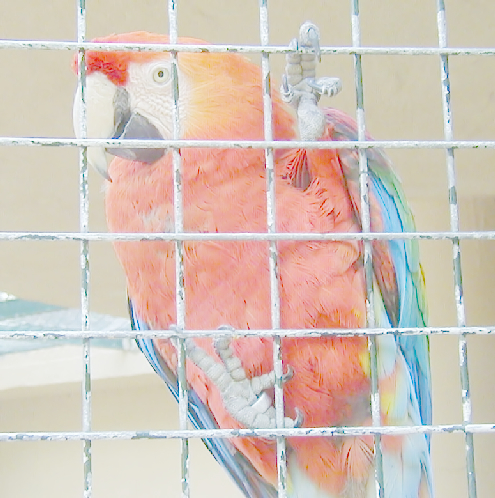
\includegraphics[scale=0.15]{./.Presentation/log}
\end{center}

\column[t]{5cm}
\begin{block}{Cortes de Color}
\justifying
Se mantienen los colores en un intervalo y se ajustan el resto de colores a un color neutral.
\end{block}
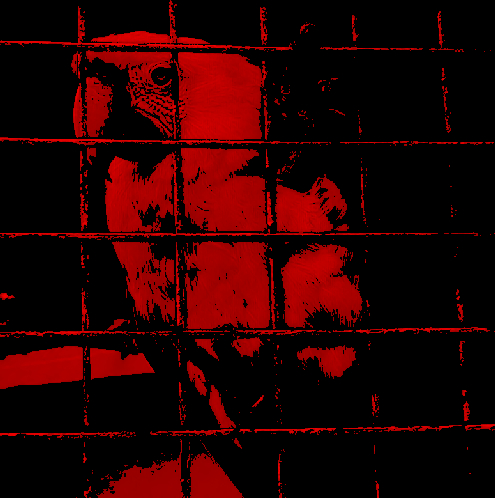
\includegraphics[scale=0.15]{./.Presentation/red}
\end{columns}

\end{frame}

\begin{frame}{Histogramas}
\begin{columns}

\column[t]{6cm}
\begin{block}{Definición}
\justifying
En una imagen, un histograma actúa como una representación gráfica de la distribución de tonos en una imagen digital. Traza el número de píxeles para cada valor tonal
\end{block}

\column[t]{4cm}
\begin{center}
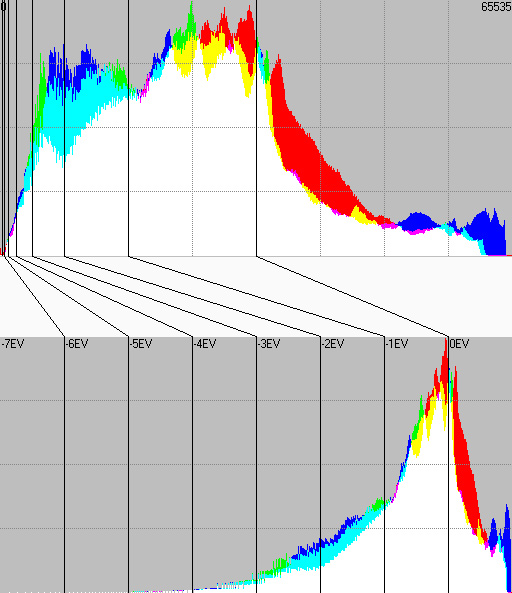
\includegraphics[scale=0.2]{./.Presentation/linlog}
\end{center}
\end{columns}
\end{frame}


\subsection{Ruidos}

\begin{frame}{Ruidos}

\begin{columns}
\column[t]{5cm}
\begin{center}
Salt\&Pepper\\
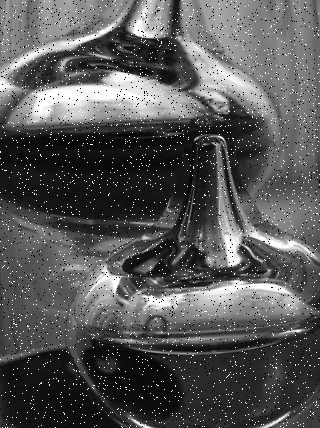
\includegraphics[scale=0.30]{./.Presentation/NoiseSP.png}
\end{center}

\column[t]{5cm}
\begin{center}
Ruido Gaussiano\\


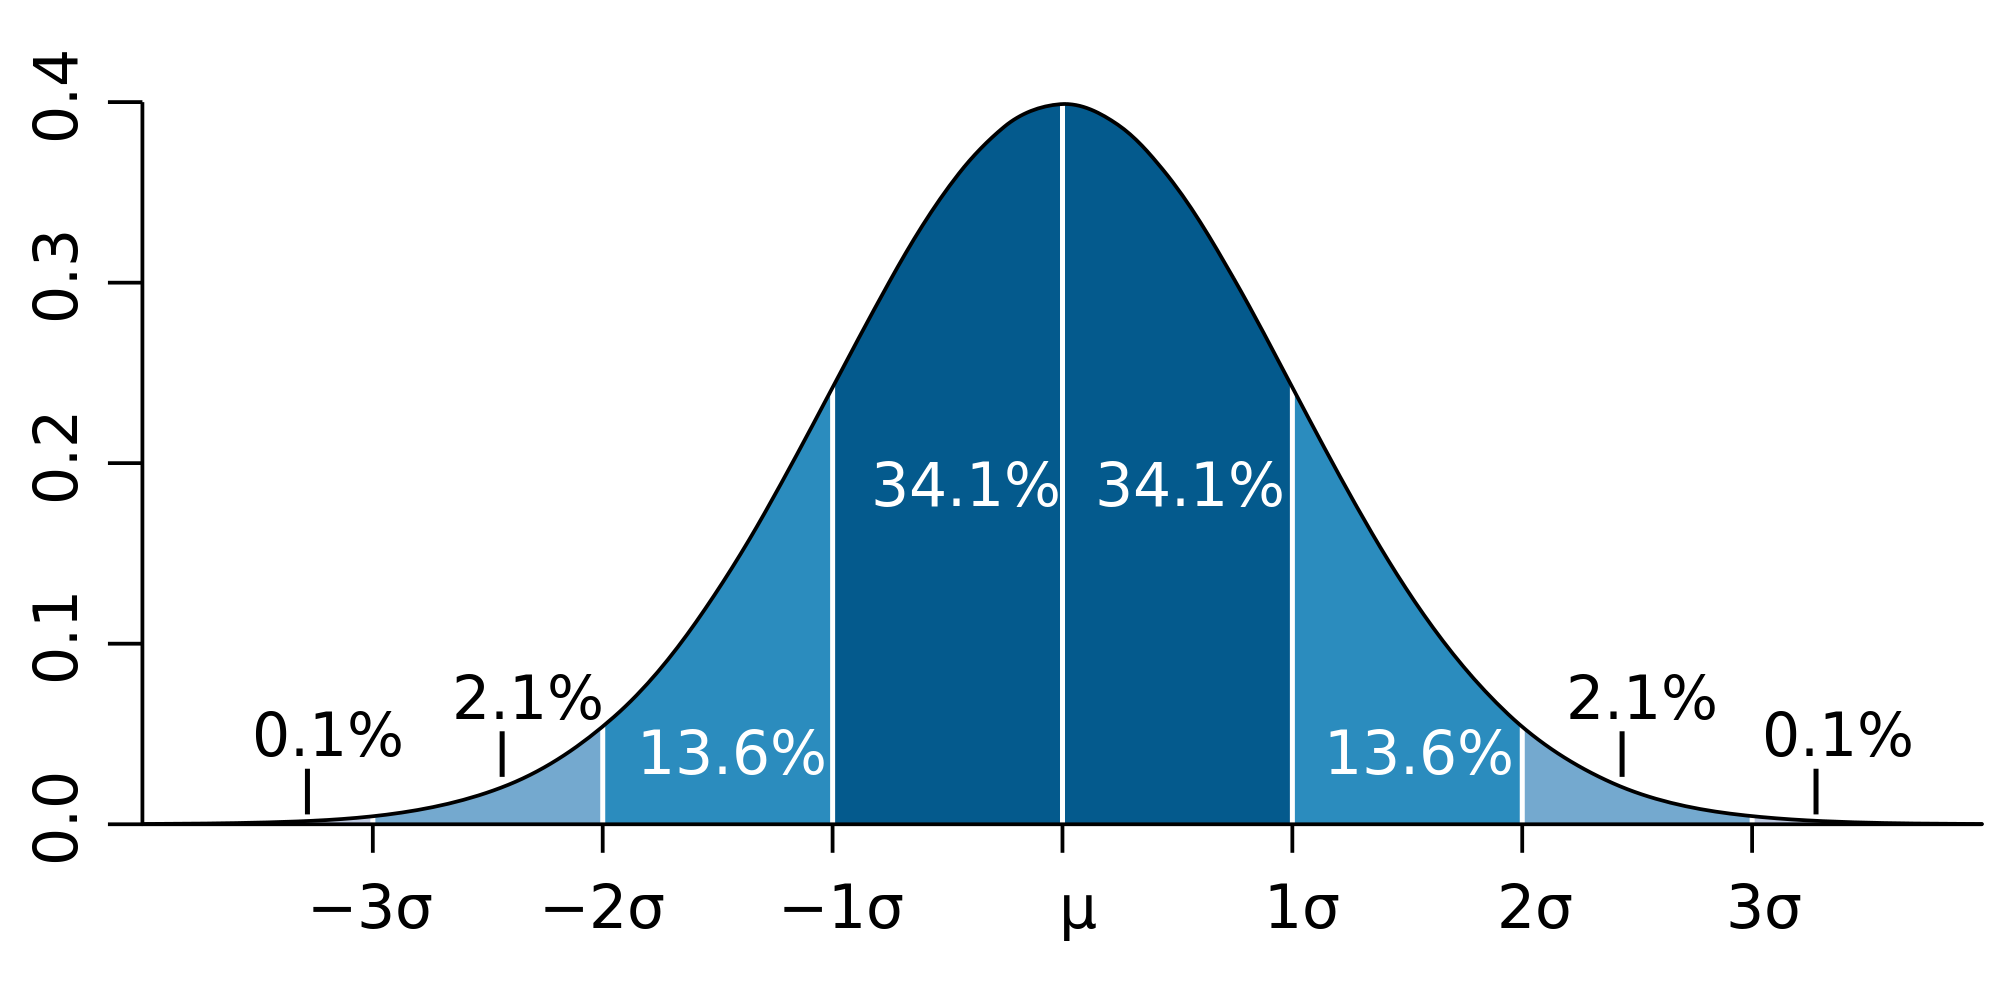
\includegraphics[scale=0.1]{./.Presentation/Standard_deviation_diagram.png}
\end{center}
\end{columns}

\end{frame}


\subsection{Otras transformaciones}


\begin{frame}{Varianza}
\begin{columns}
\column[t]{5cm}

\begin{center}
\begin{block}{Definición}
\justifying
Es una medida estadística que indica que tan alejados están los valores de la media. El filtro de varianza devuelve una imagen que contiene el cálculo de la varianza para cada pixel según sus alrededores:\\

\begin{math}
Var(x)= \frac{\sum \limits_{i=0}^{N} (\bar x - x_i)^2}{N}
\end{math}
\end{block}
\end{center}

\column[t]{5cm}

\begin{center}
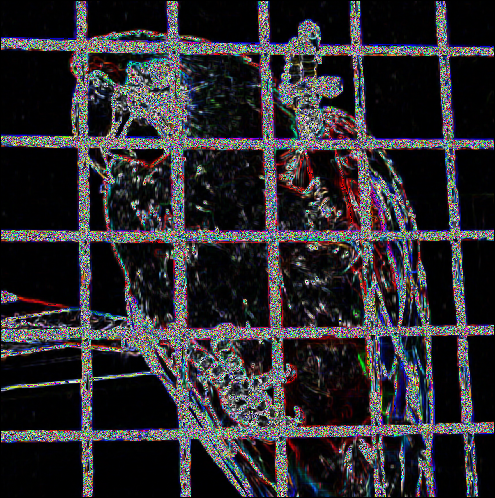
\includegraphics[scale=0.30]{./.Presentation/variance_parrot.png}
\end{center}

\end{columns}

\end{frame}

\begin{frame}{Covarianza y coorrelogramas}

\begin{block}{}
	Funciones Estadísticas.
\end{block}

Covarianza: \\

\begin{tiny}
\centering
\begin{math} 
	g(x,y) = \sum \limits_{n=0}^{N} \sum \limits_{m=1}^M \left( f(x,y) - \overline{f(x,y)}\right)\left(f(x + \Delta x, y + \Delta y) - \overline{f(x + \Delta x, y + \Delta y)} \right)
\end{math}
\end{tiny}



Correlograma: \\

\begin{small}

\begin{math}
 C_{\Delta x,\Delta y}(i,j) = \sum \limits_{p=1}^{n} \sum \limits_{q=1}^{m} 
 \left\{
	\begin{array}{l l}
		1  & \mbox{if } I(p,q)=i \mbox{  and } I(p+\Delta x,q + \Delta y)= j \\
		0 & \mbox{Otherwise}
      \end{array}\right. 
\end{math}

\end{small}

\end{frame}

\begin{frame}{Filtros Orientables: Kirsch y Freeman}

\begin{block}{Filtro Orientable}
Son filtros que se pueden aplicar para direcciones específicas.
\end{block}
\begin{columns}
\column[t]{5cm}
\begin{center}
 Kirsch Mask 0 degrees:\\

\begin{math}
   \begin{pmatrix} 
   -3 & -3 & 5 \\ 
   -3 & 0 & 5 \\
   -3 & -3 & 5 \\ 
   \end{pmatrix}
\end{math}
\end{center}

\begin{center}
 Kirsch Mask 45 degrees:\\

\begin{math}
   \begin{pmatrix} 
   -3 & 5 & 5 \\ 
   -3 & 0 & 5 \\
   -3 & -3 & -3 \\  
   \end{pmatrix}
\end{math}
\end{center}

\column[t]{5cm}
\begin{center}
 Freeman Mask 0:\\

\begin{math}
   \begin{pmatrix} 
   1 & 1 & 1 \\ 
   1 & -2 & 1 \\
   -1 & -1 & -1 \\ 
   \end{pmatrix}
\end{math}
\end{center}

\begin{center}
 Freeman Mask 1:\\

\begin{math}
   \begin{pmatrix} 
   1 & 1 & 1 \\ 
   -1 & -2 & 1 \\
   -1 & -1 & 1 \\  
   \end{pmatrix}
\end{math}
\end{center}

\end{columns}

\end{frame}








\end{document}
